%======================================================================
\chapter{Valence Bond Entanglement Entropy}
%======================================================================
\comment{SUPERNOTE: Make sure it's clear that I only did the VB EE part, not the DMRG/vN part.}

In \change{year that this happened} a new quantity called {\it{valence bond entanglement entropy}} (\vb) was proposed by \change{Fabian and co, also affleck or something?}.  
This quantity seems to have properties similar to the von Neumann entanglement entropy (\vn).
The main \change{draw, advantage} of \vb is its \change{easy to measure -ableness,
ease of measurement?} when working in the valence bond basis.
For a valence bond basis state \vb between two regions, A and B, is defined as 
\begin{equation}
\VB_A = \ln({2})\mathcal{N}_{\text{A}},
\end{equation} 
where $\mathcal{N}_{\text{A}}$ is the number of valence bonds crossing the boundary between
regions A and B.
\comment{Add in a figure showing this!!}


\vb shares some properties with \vn; in particular, for both quantities: $S_{\text{A}} = S_{\text{B}}$.
Also, $\VB = 0$ for systems with no entanglement between regions A and B.
For any single valence bond basis state \vb and \vn agree exactly, and
in one-dimensional Heisenberg spin-1/2 systems, \vb seems to to be in good agreement with
the conformal field theory (CFT) results for \vn.
However, in two dimensions \vb shows a multiplicative logarithmic correction to the area law
for the isotropic Heisenberg model.  
Ground states of unfrustrated 2D spin-1/2 systems with exclusively nearest-neighbour interactions
are expected to follow an area law \comment {reference that paper (eisert)}, though for the 2D isotropic Heisenberg model the entanglement entropy had not yet been studied \change{explicitly}.


To \change{study/examine?} \change{this quantity} and check its \change{correspondence} to a known measure of entanglement we place our \vb data alongside measurements of \vn
on the same system, calculated with density matrix renormalization group (DMRG) simulations by I. Gonzalez and R. Melko.
\vb is calculated using a single projector valence bond quantum Monte Carlo (VB QMC) scheme.

\notsay{
In 1D we fit the entanglement entropy results to the analytical results from CFT...}
\comment{Do i do an overview of what i'm going to talk about in this part?}
%-----------------------------------------------------------------------------------------------------------------------
\section{One Dimensional Systems}
%-----------------------------------------------------------------------------------------------------------------------

\change{We begin by simulating one dimensional systems, examining both the cases of
open and periodic boundary conditions.}
\notsay{The DMRG simulations require both of regions A and B to be topologically connected, so 
the same \change{convention} is used in the VB QMC simulations.}

It is convenient to denote the size of region A by the number of sites included in that region 
(i.e. for a 1D system of length $L$, $S_{\text{A}} = S(x)$ is the entanglement entropy for a system where region A contains sites $\{1,2,\dots,x\}$ and the rest of the sites $\{x+1,x+2,\dots,L\}$
belong to region B.

As mentioned in section \ref{1dcft}, for a 1D critical system the scaling of the entanglement entropy is described by CFT results as in Eq.~\eqref{cft1d}. 
\comment{Mention conformal mapping again?}

\begin{figure} {
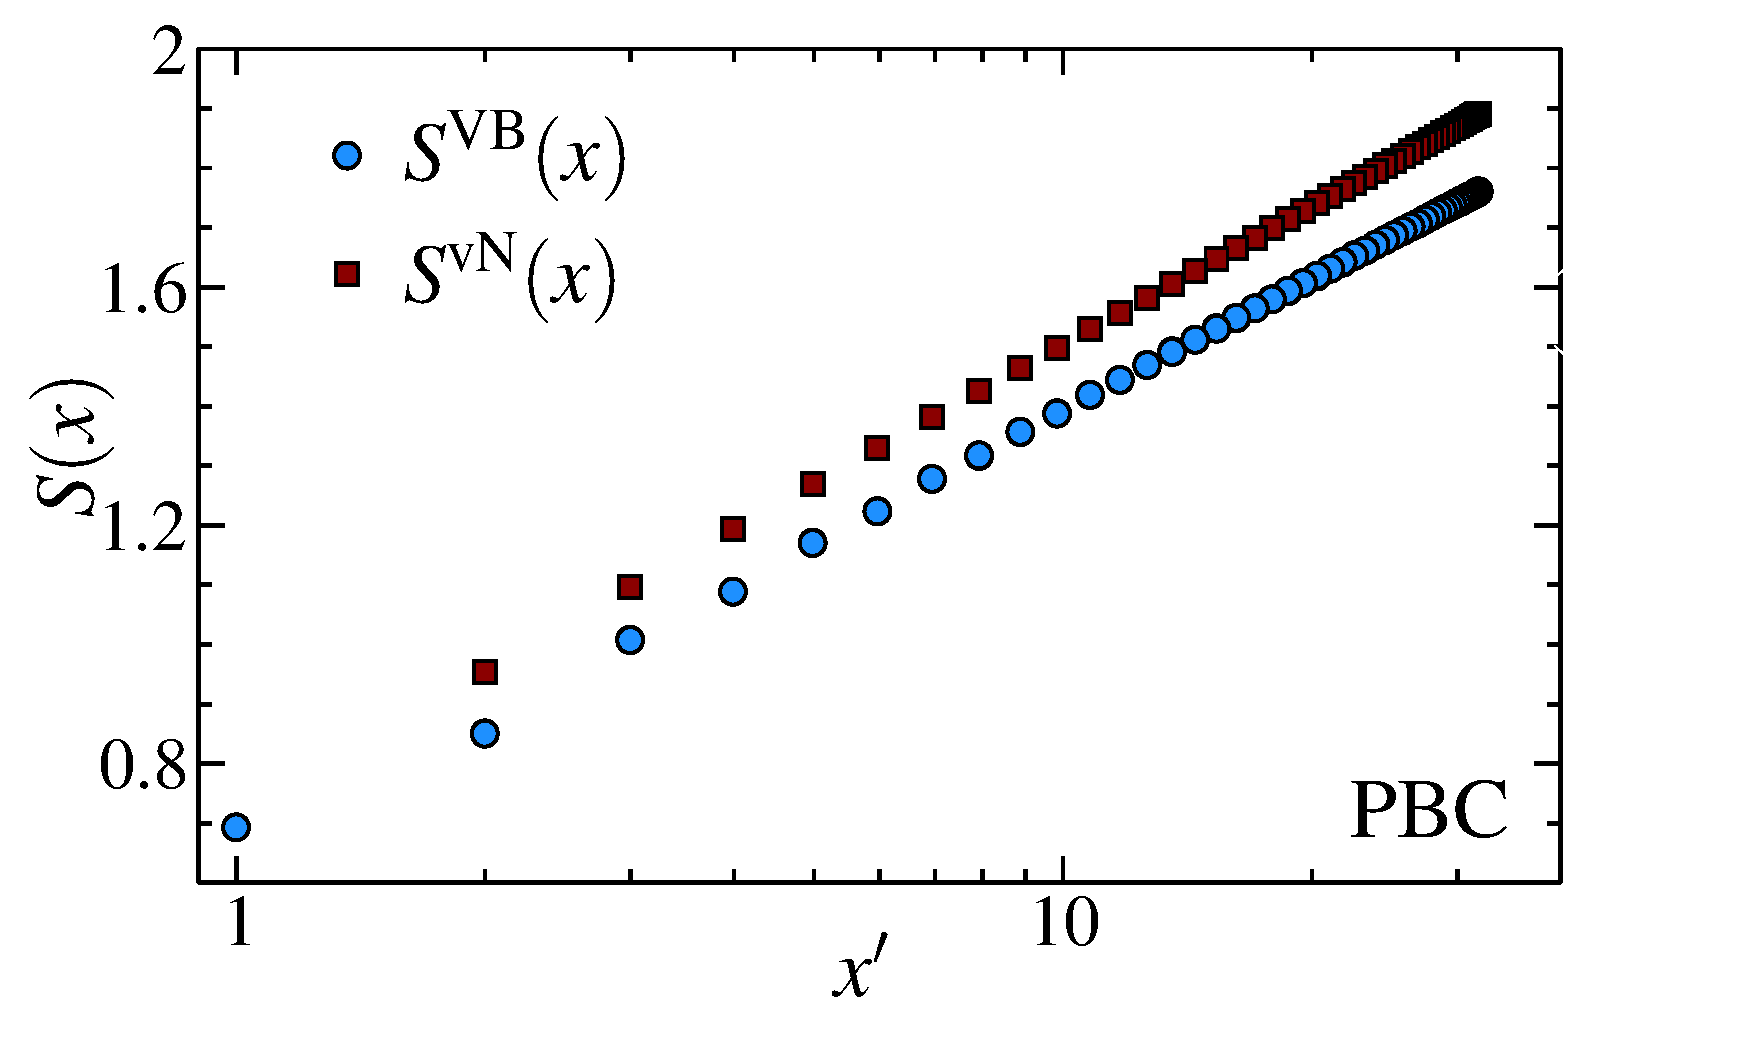
\includegraphics[width=5.5in]{./figures/paper1/figure1/thesis_pbc.eps} 
\centering
\caption[1D PBC Results for \vb with \vn]{
Entanglement entropies for a 1D, 100-site Heisenberg chain with PBC, as a function of the conformal distance $x'  = (L/\pi)\sin (\pi x/L)$.
\label{1dPBC}}
} 
\end{figure}

Figure \ref{1dPBC} shows the \vb measurements for a periodic spin chain with 100 sites, plotted alongside \vn data.  \vb seems to fit well to the CFT result, though it is lower than \vn.
Linear regression fits of the \vb and \vn data for several system sizes (Figure~\ref{c1}) shows $c^{\rm vN}$ approaching 1 as the system size increases, however $c^{\rm VB}$ gives a lower value of $c$.


\begin{figure} {
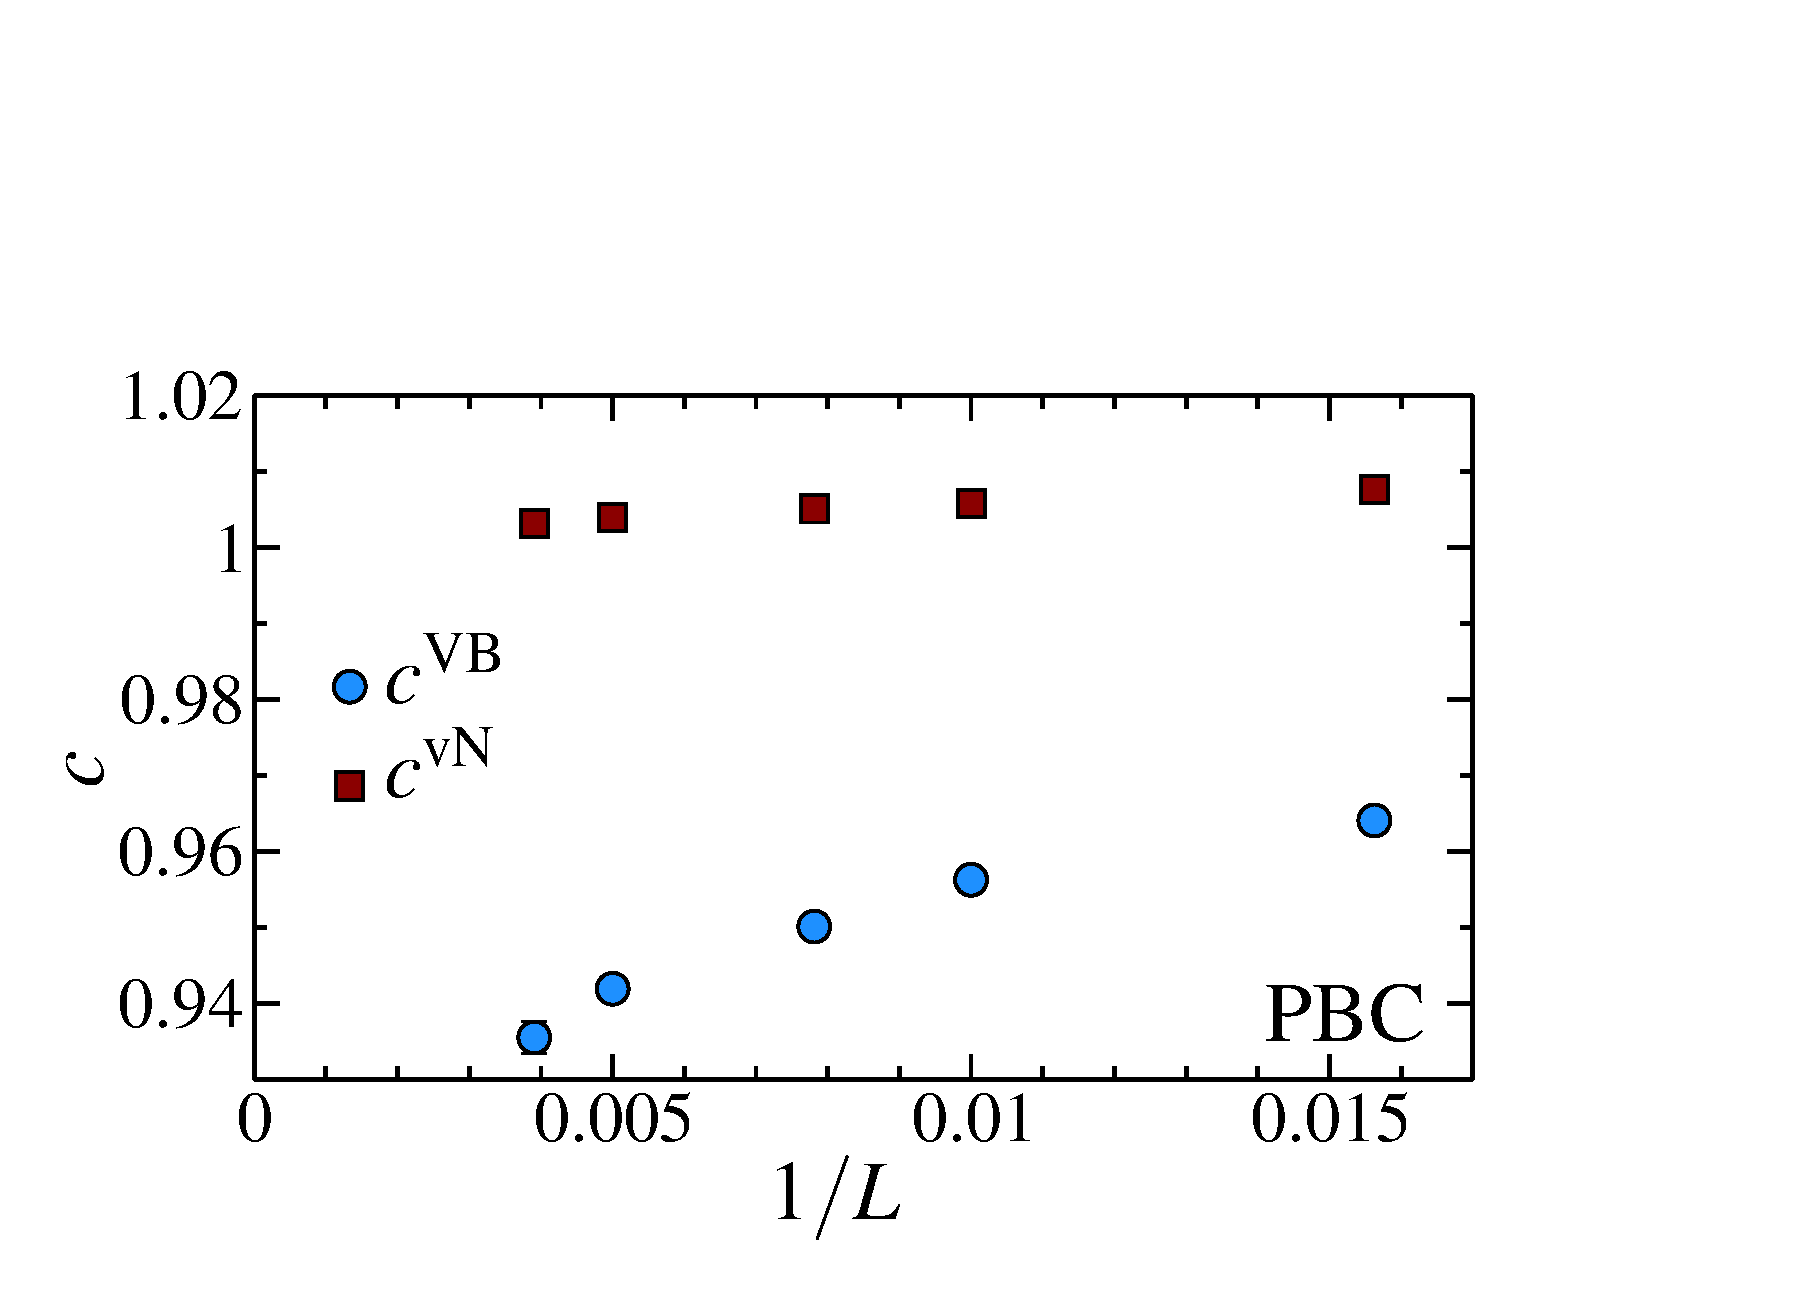
\includegraphics[width=6in]{./figures/paper1/figure1/thesis_c1.eps} 
	\centering
	\caption[1D Results for VB EE and von Neumann EE]{
	The central charge, $c$, found using linear regression fits of the entanglement entropy data 	for periodic Heisenberg chains for length L=64, 100, 128, 200, and 256.  Data for the two smallest 	points ($S(1)$ and $S(L-1)$) are removed for the calculation of $c$ \notsay{since the DMRG data 	do not include these region A sizes}.
	\label{c1}}
} 
\end{figure}


\begin{figure} {
	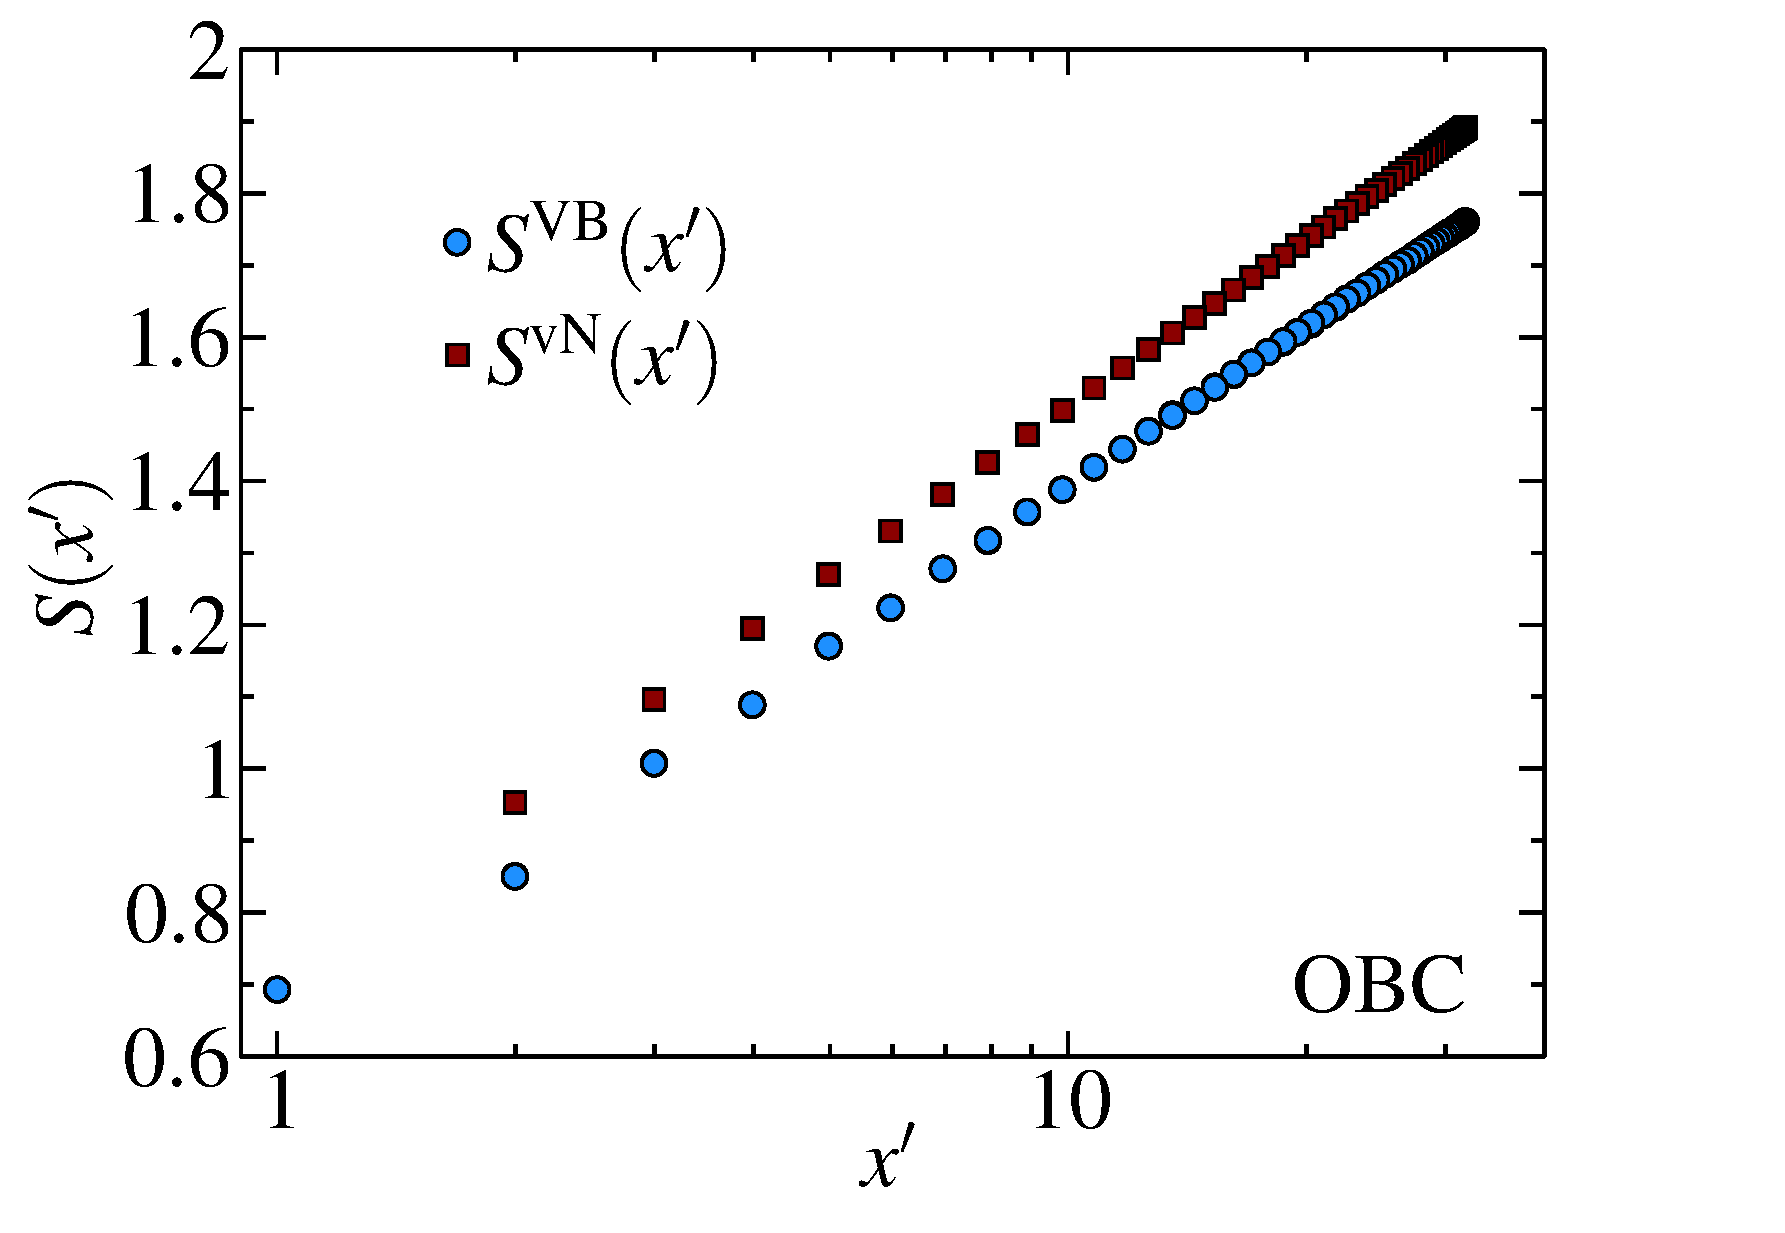
\includegraphics[width=5.5in]{./figures/paper1/figure1/thesis_obc.eps} 
	\centering
	\caption[1D OBC Results for VB EE and von Neumann EE]{
	Entanglement entropies for a 1D 100-site Heisenberg chain with OBC as a function of the conformal distance $x'  = (L/\pi)\sin (\pi x/L)$.
	\label{1dOBC}}}
\end{figure}

\change{For the OBC case} (Figure~\ref{1dOBC}), we see entanglement entropies split into two branches, where the upper branch corresponds to an odd number of sites in region A, and the lower to an even number.
\change{This branching is due to a ``dimerization" effect caused by the open boundary conditions \cite{Ian1}.}
In contrast to the PBC case, \vb is now higher than \vn.

\begin{figure} {
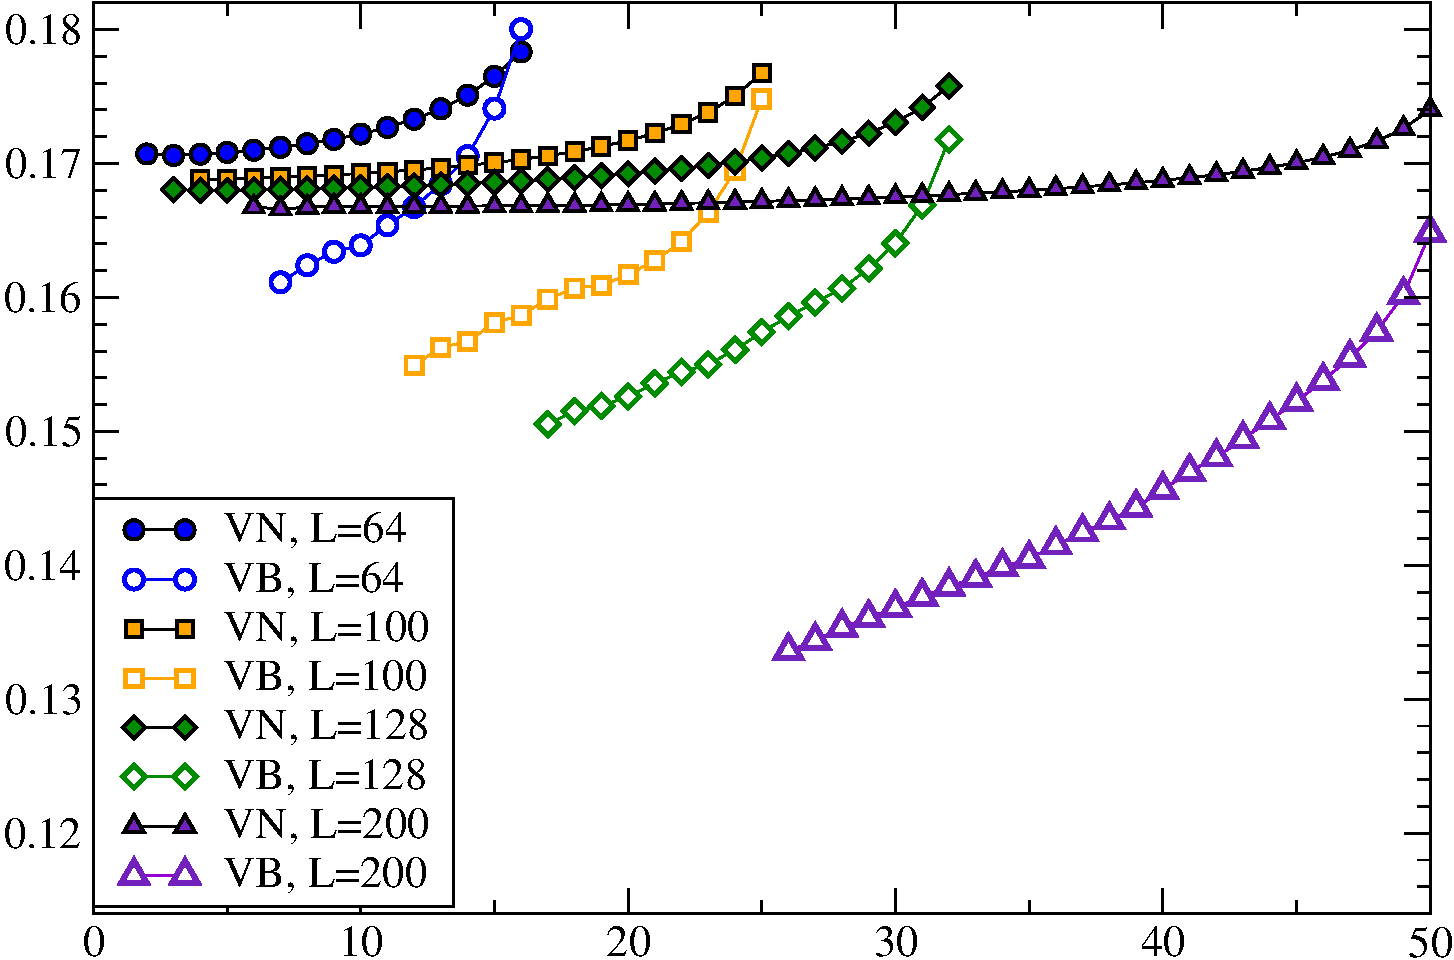
\includegraphics[width=6in]{./figures/paper1/figure1/fig2_NEW.eps} 
\centering
\caption[caption]{ 
	caption
}}
\end{figure}

\comment{Totally talk about $c$ for the OBC case.}

%------------------------------------------------------------------------------------------------------------------
\section{Approaching Two Dimensions}

\comment{make a diagram of the snaking pattern for the dmrg!}
 
\begin{figure} { 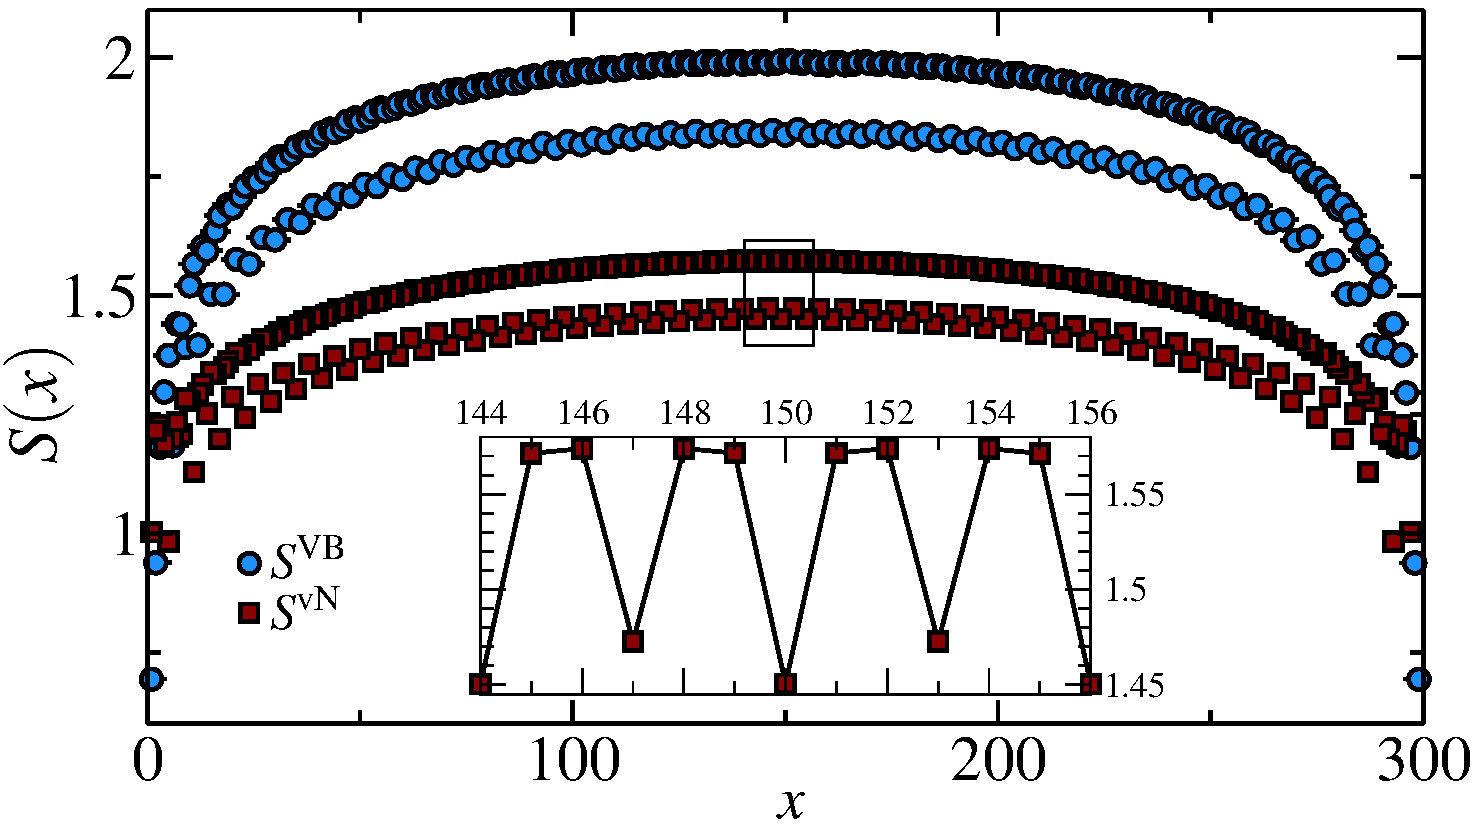
\includegraphics[width=6in]{./figures/paper1/figure3/3-leg-ladder/fig3_final2.eps}
\caption[Entanglement entropies for a three-leg ladder]{
Entanglement entropies for a three-leg ladder with OBC and 100 sites per leg.  
The inset shows a close up view of the boxed region.
 \label{ladder3} }} 
 \end{figure}
 
 \begin{figure} { 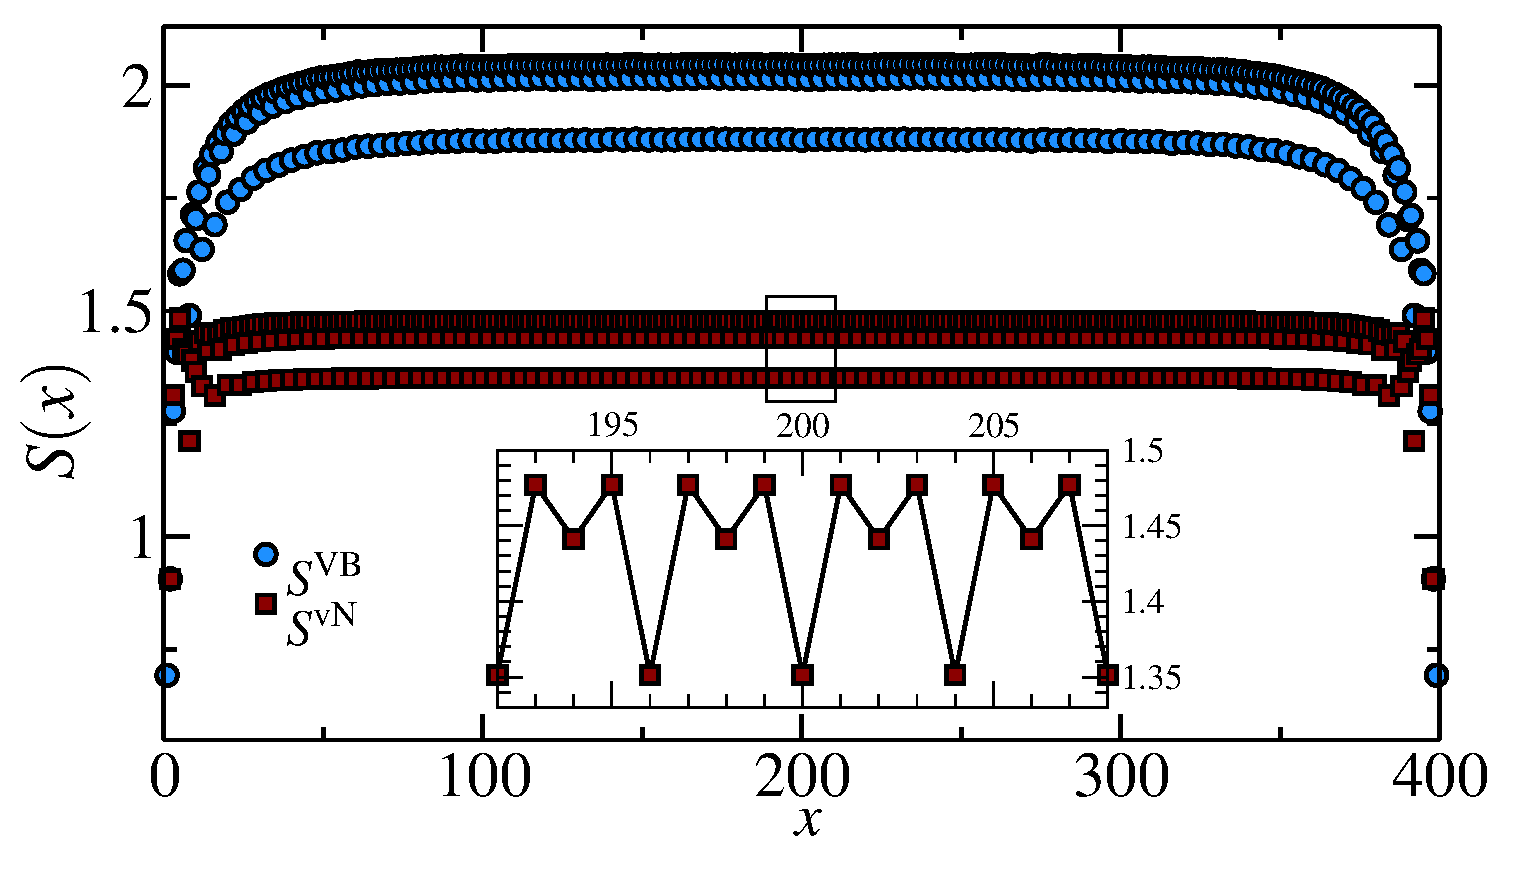
\includegraphics[width=6in]{./figures/paper1/figure3/4-leg-ladder/4legfig.eps}
\caption[Entanglement entropies for a four-leg ladder]{
Entanglement entropies for a four-leg ladder with OBC and 100 sites per leg.  
The inset shows a close up view of the boxed region.  
 \label{ladder4} }} 
 \end{figure}
 
 We now move towards two dimensions by adding ``legs" to our one dimensional chains.
 Due to the constraints imposed by the DMRG on the geometry of region A the sites must be arranged in a snaking pattern. \comment{(See Figure)}
The DMRG data, to which we compare \vb, are limited to ladders with $M=7$ legs because of the \change{poor scaling of the algorithm when approaching 2D}.
 The VB QMC algorithm \change{scales as $N^2$} for a system with N sites, so \change{ we measure up to $M=20$ with minimal CPU effort}.
 
 Figures \ref{ladder3} and \ref{ladder4} show the entanglement entropies for three- and four-leg ladders respectively.
 As with the 1D OBC spin chain, $\VB > \VN$ for these $M$-leg ladders.
 \vn and \vb show different behavior depending on whether the number of legs is even or odd.
 For odd-leg ladders
 
 \notsay{
 For ladders with an even number of legs, away from the open boundaries $S = \text{const}$.}
 
 \comment{Say something about the ``spin gap"? White, Noack, Scalapino, 1994.}
 
%------------------------------------------------------------------------------------------------------------------
\section{The Area Law}

\begin{figure} { 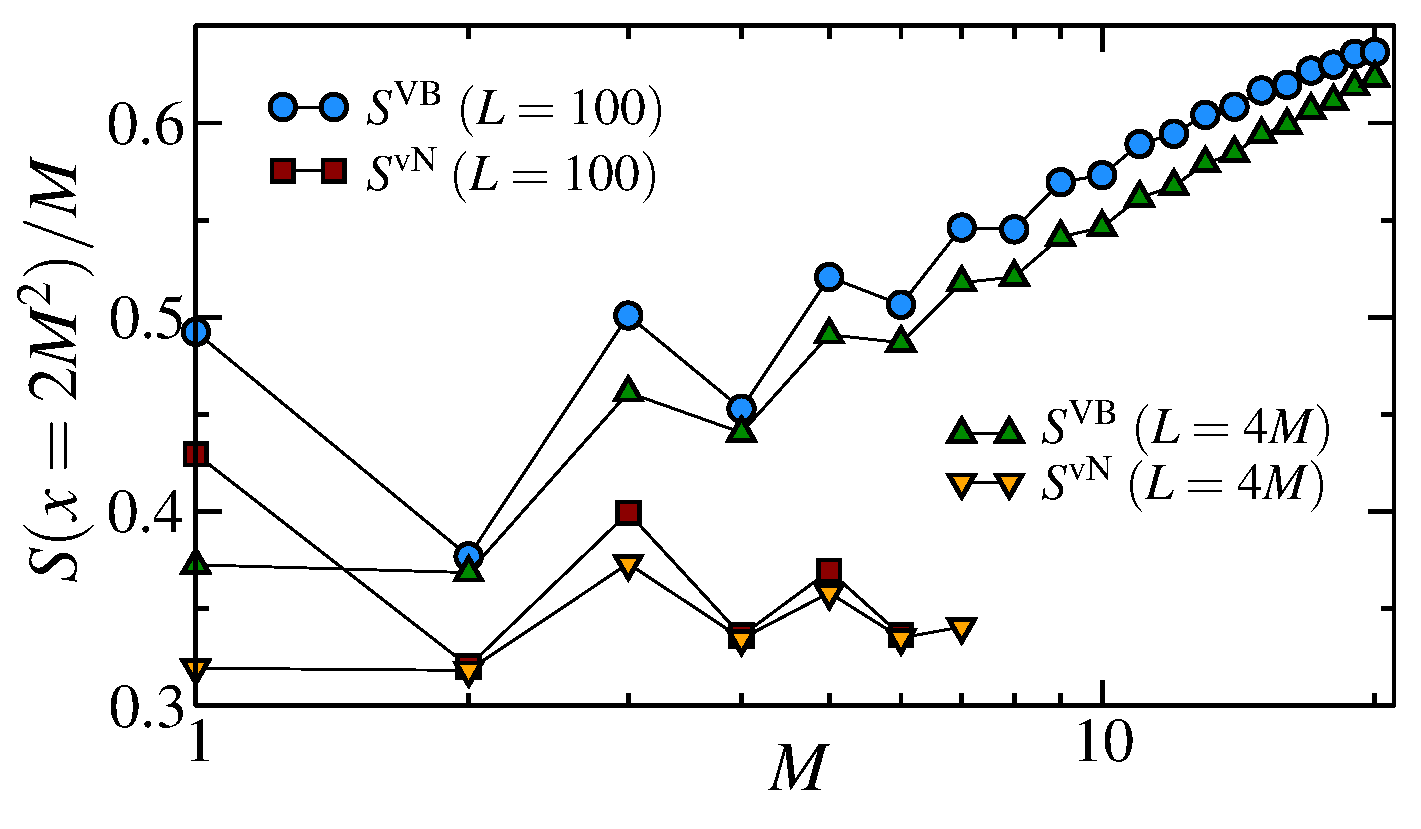
\includegraphics[width=6in]{./figures/paper1/figure4/4fig.eps}
 \caption[Area Law in 2D Heis model]{
Entanglement entropies divided by $M$,  for $M$-leg ladders, taken such that
the region A includes $2M^2$ sites.  
Data from both ladders of  with $L=100$ sites per leg and ladders of length $L=4M$ 
\notsay{(with length proportional to the number of legs)} are shown.
For large $M$, $S^{\rm VB}\propto M \ln M$,
whereas $S^{\rm vN}\propto M$.   
\label{zigzag}}} 
\end{figure}
%------------------------------------------------------------------------------------------------------------------
\comment{\section{Analytical Calculations?}}